\documentclass[10pt,conference]{IEEEtran}

\usepackage{booktabs}
\usepackage{amsmath}
\usepackage{amssymb}
\usepackage{amstext}
\usepackage{graphicx}

\usepackage{tabularx}
\usepackage{array}

\graphicspath{{figures/}}

\usepackage[T1]{fontenc}
\usepackage{cite}
\usepackage{xspace}
\usepackage{url}

\usepackage[hidelinks]{hyperref}
\setlength{\textfloatsep}{3pt plus 1pt minus 1pt}
\setlength{\floatsep}{3pt plus 1pt minus 1pt}
\renewcommand{\topfraction}{0.98}
\renewcommand{\textfraction}{0.02}
\renewcommand{\floatpagefraction}{0.9}
\setcounter{topnumber}{3}
\setcounter{totalnumber}{5}

\newcommand{\sysname}{TraceAssist\xspace}
\newcommand{\uu}[1]{\,\textsf{#1}}

\title{TraceAssist: Answering Kernel Trace Questions in Natural Language}

\author{
\IEEEauthorblockN{Sneh Patel\IEEEauthorrefmark{1},
Yuvraj Sehgal\IEEEauthorrefmark{1},
Mahsa Panahandeh\IEEEauthorrefmark{2},
Naser Ezzati-Jivan\IEEEauthorrefmark{1},
Francois Tetreault\IEEEauthorrefmark{3}}
\IEEEauthorblockA{\IEEEauthorrefmark{1}Department of Computer Science,
Brock University, St.\ Catharines, Ontario, Canada\\
\IEEEauthorrefmark{2}School of EECS, University of Ottawa, Ottawa,
Ontario, Canada; \IEEEauthorrefmark{3}Ciena Corporation, Ottawa, Canada\\
\{sp18oo, ys19rk, nezzatijivan\}@brocku.ca, mpanahan@uottawa.ca,
ftetreau@ciena.com\\[1pt]
{\scriptsize S.~Patel: \url{https://www.researchgate.net/profile/Sneh_Patel16}}\\
{\scriptsize Y.~Sehgal: \url{https://17yuvrajsehgal.github.io/Yuvraj-Portfolio-Website/}}\\
{\scriptsize M.~Panahandeh: ORCID \url{https://orcid.org/0000-0002-6369-8982};
N.~Ezzati-Jivan: ORCID \url{https://orcid.org/0000-0003-1435-6297}}}
}

\begin{document}
\maketitle
\begin{abstract}

Large Language Models (LLMs) have difficulty answering questions about execution traces that exceed their context limits or that contain unfamiliar system behaviour. Retrieval-augmented generation (RAG) provides relevant documentation but cannot establish what happened during a specific execution. We present \sysname, a framework for answering natural language questions about Linux kernel traces. Analyzers built on Trace Compass compute findings from the whole trace, RAG supplies domain and program documentation, and an LLM explains the evidence in natural language. We evaluated \sysname on 2, 10, and 30 minute LTTng traces of a multithreaded program with one slow thread, using 13 questions covering comprehension, root cause, dependencies, quantitative analysis, and remediation. Using GPT-5.6, baselines given raw trace excerpts or excerpts with RAG score 35\% and 68\%, respectively. \sysname answers every question correctly across all three traces, with timings matching measured ground truth. These results suggest that combining computed trace evidence with retrieved documentation can support performance diagnosis through natural-language questions.
\end{abstract}

% \begin{IEEEkeywords}
% large language models, retrieval-augmented generation, execution traces,
% LTTng, Trace Compass, performance analysis
% \end{IEEEkeywords}


\section{Introduction}

Large language models (LLMs) now sit inside search engines, editors and developer tools. They are reliable for knowledge that is common on the web. However, they struggle with information that is too large to process effectively, where accuracy can drop even before the context limit is reached~\cite{liu2024lost}. Another challenge is rare or private information, such as a company's internal systems, that is poorly represented or absent from their training data~\cite{kandpal2023longtail}. In both cases, models can fill the gaps with convincing but unsupported claims~\cite{ji2023hallucination}.

Execution traces combine both problems. A kernel tracer such as LTTng~\cite{desnoyers2006lttng} records every system call, scheduling decision and interrupt; a 30-minute trace of the program we study holds approximately 87 million events, far beyond any context window. And a developer's question, such as \textit{why one thread is slow}, concerns one specific program that appears in no training corpus. Tools such as Trace Compass~\cite{tracecompass} can answer it, but requires domain specialized domain knowledge. 

Retrieval-augmented generation (RAG)~\cite{lewis2020rag} retrieves relevant documents and adds them to the prompt. These documents can explain concepts and program design, but do not establish what happened during a particular execution. For example, RAG can explain what a \texttt{futex} wait is, but determining how long a thread waited or which thread woke it requires evidence from the trace.

We present \sysname, a framework that answers natural language questions about kernel traces using computed evidence and relevant documentation. Each question guides the selection of analyzers built on Trace Compass and the threads they examine. These analyzers produce measured findings, such as how a thread's time is divided between running, waiting for CPU and being blocked, or which other threads wake it. RAG supplies domain and program documentation, and an LLM combines this context with the findings to explain the answer.  Our contributions are:

\begin{itemize}
    \item \sysname, a framework that grounds answers in question-guided trace analysis, uses RAG to supply relevant documentation, and employs an LLM to explain the findings.
    \item A benchmark comprising LTTng traces of a multithreaded program with one slow thread, recorded at three durations, and 13 questions spanning five categories with measured ground truth.
    \item An evaluation using the same LLM across all approaches: raw trace excerpts and excerpts with RAG yield scores of 35\% and 68\%, respectively, while \sysname answers all 13 questions correctly on every trace.
\end{itemize}

\section{Related Work}

TAAF~\cite{ezaz2026taaf} is the work closest to ours. It answers natural-language questions about LTTng kernel traces by building a time-indexed Trace Compass state system and, for each question, extracting a knowledge graph of threads, CPUs and resources, over which an LLM reasons. On TraceQA-100, 100 questions about slices of a SciMark~2.0 trace, it improves accuracy by up to 31.2\% over the state system's numeric output, mostly on multi-hop and causal questions; our hub-scope labels follow its distinction between single- and multi-hop questions. \sysname differs in three ways. Its analyzers compute the measurements an answer needs, such as wait chains and per-round finish times, so the LLM explains results rather than deriving them from a graph. It analyzes whole traces rather than slices; our evaluation uses traces lasting up to 30 minutes, whereas TAAF evaluates slices of at most 100\,s. It also adds retrieved documentation to the trace evidence.

Outside kernel tracing, two systems share \sysname's division of labour between deterministic evidence gathering and LLM explanation. RCACopilot~\cite{chen2024rcacopilot} matches each cloud incident at Microsoft to a handler that collects diagnostic data, then has an LLM predict the root-cause category and explain it, reaching an accuracy of up to 0.766 on a year of incidents. Opal~\cite{zaeed2025opal} adds hardware-counter and Roofline analytics to LLM prompts to optimize GPU kernels; even a single source of insight produced a speedup in over 98.5\% of 1{,}640 experiments, and its one incorrect result stemmed from a vague diagnostic, which supports giving the LLM precise findings. \sysname brings this design to kernel traces, where the evidence must first be computed from millions of events, and to open questions rather than classification or code generation.


\section{Methodology}

\begin{figure}[t]
\centering
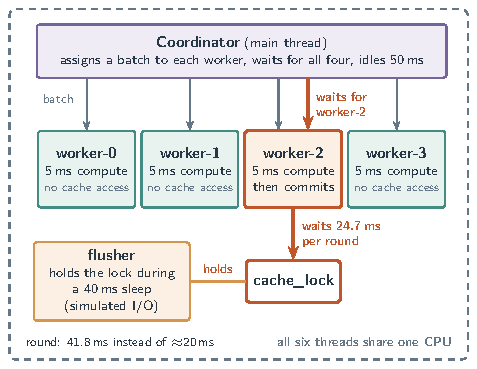
\includegraphics[width=\columnwidth]{batch_server}
\caption{The \texttt{batch\_server} workload. The coordinator waits for all four workers; \texttt{worker-2} must acquire \texttt{cache\_lock}, which \texttt{flusher} holds during a 40\,ms simulated I/O, so lock contention delays \texttt{worker-2} and the whole round.}
\label{fig:batchserver}
\end{figure}

We wrote a C program \texttt{batch\_server} (Fig.~\ref{fig:batchserver}), with a known performance bug. The program executes approximately 11 rounds per second. In each round, a coordinator thread assigns work to four worker threads, each performing about 5\,ms of computation, waits for all workers to finish, and then idles for 50\,ms. One worker \texttt{worker-2}, also commits its results to a shared cache protected by a mutex, \texttt{cache\_lock}. A separate \texttt{flusher} thread holds this lock while writing the cache back, with slow I/O simulated by a 40\,ms sleep. All six threads share one CPU. Holding the lock during this simulated I/O causes \texttt{worker-2} to wait an average of 24.7\,ms per round to acquire it. As a result, the work phase takes 41.8\,ms instead of the roughly 20\,ms needed for four 5\,ms computations on one CPU. The program logs timings for each round to provide ground truth.

We traced the program system-wide with LTTng kernel tracing (system calls, scheduling, timers and interrupts) for 2, 10 and 30 minutes, giving traces of  5.9, 29.3 and 86.9 million events (1{,}305, 6{,}528 and 19{,}580 rounds). Activity from the rest of the machine stays in the traces, as it would in practice. Three systems, all using GPT-5.6 through the OpenAI API, answer the same questions about each trace.

\subsection{Baseline 1: LLM Only}

The first baseline tests whether a capable LLM can answer from the trace itself, with no tools. Each trace is printed as text with \texttt{babeltrace2}, one line per event. Even the 2-minute trace has 5.9 million events, about 380 million tokens, far beyond the model's context window, so the model receives a \emph{slice} of at most 200{,}000 tokens (about 3{,}000 events). What the model can answer depends on which part of the trace it sees, so we cut the slice in three ways, each modeling a way a user might shorten a trace; the ranges below span the three traces. \textbf{(A)~Head:} the first 200k tokens, as if the user pasted the trace into a chat and it was cut off at the limit. Because tracing starts before the program does, this covers only the first 4.7--5.7\,ms and contains no events from the program, testing what the model does without relevant evidence. \textbf{(B)~Middle:} 200k tokens of consecutive events from the trace's midpoint, as if the user had picked a moment when the program was running. It spans 96--125\,ms, about one round, so the model sees one complete, detailed instance of the slowdown but nothing of the other rounds. \textbf{(C)~Sampled:} 20 windows of 10k tokens spread evenly across the whole trace (every 6, 30 or 90\,s on the three traces), each labeled with its time range. Each window typically covers only 6--11\,ms, shorter than a round, so the model sees fragments of many rounds rather than one whole round: breadth instead of depth.

A header gives the full trace's length and says that most events are omitted. The system prompt asks the model to act as a Linux tracing expert, answer only from the trace text, name threads, thread IDs, CPUs and durations, and say when the text is not enough. Each question is a separate API call, so no answer can draw on another, and questions name threads by name only. The model never sees the ground-truth files. With 13 questions, 3 slices and 3 traces, each baseline produces 117 answers.

\subsection{Baseline 2: LLM with RAG}

The second baseline adds RAG to the first and changes nothing else. Its knowledge base holds 38 documents: 15 on Linux kernel tracing concepts, such as futex waits, thread states and wake-ups; 12 on Trace Compass analyses; 10 other documents unrelated to the program, which act as distractors; and a description of \texttt{batch\_server}, standing in for the internal documentation an organization keeps for its own software. It names the threads and \texttt{cache\_lock} and states the design, including that the flusher sleeps for 40\,ms while holding the lock, so it points to the likely root cause, as such documentation would in practice. It contains no measurements of any run, so it cannot supply the measured answers, such as how long \texttt{worker-2} waits per round or how much faster rounds would be after a fix; those must come from the trace. \sysname uses the same 38 documents, so the documentation is not what separates the two systems.

Documents are embedded with \texttt{bge-small-en-v1.5} and stored in ChromaDB. The question is the search query: the six nearest documents are kept, and the top three are expanded to their full text. \sysname uses the same index and expansion but different queries: each concept its findings name, such as the program, the system call a thread blocked in, or a wait chain, first retrieves its best-matching document, and the question fills the remaining places. The retrieved documents are fixed per question; the program description was retrieved for 10 of the 13 questions, ranked first for 6. The system prompt instructs the model to derive facts about the execution from the trace text and use the documents only to interpret those facts. An answer that merely repeats the program description without supporting evidence from the trace slice receives half credit.

\subsection{\sysname}

\begin{figure*}[t]
\centering
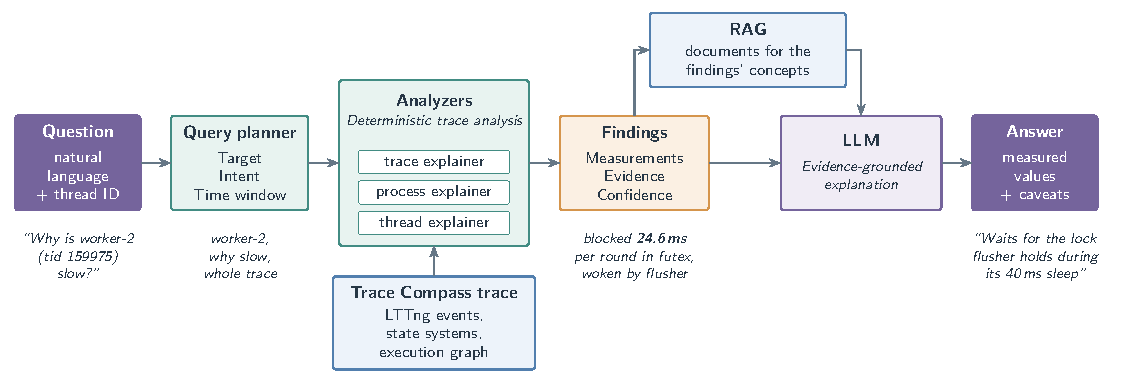
\includegraphics[width=\textwidth]{traceassist_pipeline}
\caption{\sysname's pipeline from question to answer: deterministic trace analysis produces the findings, and the LLM explains them. The italic text follows one question, Q5 on the 2-minute trace, through each step.}
\label{fig:pipeline}
\end{figure*}

\sysname has four components (Fig.~\ref{fig:pipeline}): a query planner, a set of analyzers, a retrieval step and an LLM, packaged as a Trace Compass plug-in. The query planner uses rules, not the LLM, to choose the target (a thread, a process or the whole trace), the intent, such as explaining where a thread's time went, and the time window; when a question names a time range, the detailed analysis is limited to it. The LLM, the same GPT-5.6 model as in both baselines, never reads the trace's events: beyond the trace's name and time range, it sees only the plan, the findings and the retrieved documents.

\textbf{Analyzers.} Three analyzers, built on Trace Compass's kernel state system and execution graph, cover the three targets:
\begin{itemize}
  
  \item The \emph{trace explainer} summarizes the trace: which events were recorded, which processes ran and used the CPU, and which are the workload rather than background activity or the tracer.
  
  \item The \emph{process explainer} splits each thread's time into running, waiting for CPU and blocked, follows the execution graph's wake-up edges to find which thread ended each wait, and names the bottleneck: the thread the main thread waits on, with its wait chain to the root (here main thread $\leftarrow$ \texttt{worker-2} $\leftarrow$ \texttt{flusher} $\leftarrow$ timer). Over every round it measures when each thread finishes, how long the lock holder holds the lock, inferred from the waits and wake-ups around it, and how long rounds would take without the bottleneck's wait.
  
  \item The \emph{thread explainer} splits one thread's time by state and explains each large share: for blocked time, the system call and the critical path to the thread that ended the wait; for CPU waits, which threads held the CPU; for running time, user and system time. It also adds the thread's part in its process's recurring wait chain, so that a one-off wait, such as the startup pause, is not mistaken for the recurring cause.
  
\end{itemize}
Each analysis result is stored as a JSON object called a \emph{finding}. It contains a one-sentence summary, supporting measurements, the time window covered, the evidence used, a confidence level and any limitations. Conclusions drawn from indirect evidence, such as which thread held a lock, are marked as medium confidence. The LLM's rules require every statement about the trace to come from a finding, with its numbers, and a missing finding to be stated rather than guessed. An auxiliary statistical module, TMLL, adds system-call summaries; we leave its evaluation to future work.

\textbf{Protocol and limitation.} \sysname currently identifies the thread a question asks about by its ID, as in \texttt{Why is worker-2 (tid 164857) slow?}. A name resolver handles process names and uniquely named threads, but threads that share a name, as in a thread pool, still need the ID, so our thread questions carried it; the baselines' questions did not. Removing this dependence is future work. For each trace, \sysname answered Q1--Q10 and Q11--Q13 in two separate conversations, retaining context within each conversation and producing 39 answers in total.

\section{Evaluation}


% \begin{table*}[t]
% \centering
% \caption{The 13 questions, their category and hub scope, and each system's score. Baselines: one answer per slice (A, B, C) for each of the three traces, so 9 per question. \sysname: one answer per trace, so 3 per question. Correct = 1, partly correct = \textonehalf, wrong = 0.}
% \label{tab:questions}
% \small
% \setlength{\tabcolsep}{4pt}
% \begin{tabularx}{\textwidth}{@{}r>{\raggedright\arraybackslash}Xllrrr@{}}
% \toprule
% Q & Question & Category & Hub scope & LLM (/9) & RAG (/9) & \sysname (/3) \\
% \midrule
% 1  & What does this trace record? & Comprehension & Multi & 3 & 2.5 & 3 \\
% 2  & What does each thread of \texttt{batch\_server} do? & Comprehension & Multi & 3 & 7.5 & 3 \\
% 3  & Which CPU(s) does \texttt{batch\_server} run on? & Comprehension & Single & 6 & 7.5 & 3 \\
% 4  & Which thread is the bottleneck of \texttt{batch\_server}? & Root cause & Multi & 2 & 7.5 & 3 \\
% 5  & Why is \texttt{worker-2} slow? & Dependency & Multi & 1 & 7.5 & 3 \\
% 6  & Is \texttt{worker-2} slow because it uses more CPU than the other workers? & Dependency & Multi & 4 & 5.5 & 3 \\
% 7  & What is \texttt{worker-2} waiting on, and which thread wakes it up? & Dependency & Single & 5.5 & 6.5 & 3 \\
% 8  & Why does \texttt{flusher} hold the lock for so long? & Dependency & Single & 1 & 7.5 & 3 \\
% 9  & Break down how \texttt{worker-2} spends its time in a typical round. & Quantitative & Single & 2 & 2 & 3 \\
% 10 & What change would fix the slowdown, and how much faster would rounds be? & Remediation & Multi & 0 & 7.5 & 3 \\
% 11 & In a typical round, how much later does \texttt{worker-2} finish than the other workers? & Quantitative & Multi & 2 & 5.5 & 3 \\
% 12 & How could \texttt{flusher} hold \texttt{cache\_lock} for less time, and how long afterwards? & Remediation & Single & 6.5 & 7.5 & 3 \\
% 13 & Does another thread hold up \texttt{flusher}, or does it delay itself? & Root cause & Single & 5.5 & 5.5 & 3 \\
% \midrule
%    & \textbf{Total} & & & 41.5/117 & 80/117 & 39/39 \\
%    & & & & (35.5\%) & (68.4\%) & (100\%) \\
% \bottomrule
% \end{tabularx}
% \end{table*}

\begin{table}[t]
\centering
\caption{Points scored out of the maximum possible, with the percentage; each answer scores 1, \textonehalf{} or 0. The maximum is the number of answers a row covers. A slice row covers all 13 questions on the three traces, so 39 answers. A category or hub-scope row covers only its questions, each answered 9 times by a baseline (3 slices $\times$ 3 traces) and 3 times by \sysname (once per trace): comprehension, for example, has 3 questions, so 27 and 9. \sysname reads the whole trace, so it has no slices.}
\label{tab:breakdown}
\footnotesize
\setlength{\tabcolsep}{2pt}
\begin{tabular}{@{}lrrr@{}}
\toprule
 & LLM & RAG & \sysname \\
\midrule
Slice A (head)   & 1.5/39 (4\%)   & 11.5/39 (29\%) & -- \\
Slice B (middle) & 21.5/39 (55\%) & 35/39 (90\%)   & -- \\
Slice C (sampled)& 18.5/39 (47\%) & 33.5/39 (86\%) & -- \\
\midrule
Comprehension         & 12/27 (44\%)   & 17.5/27 (65\%) & 9/9 (100\%) \\
Root cause            & 7.5/18 (42\%)  & 13/18 (72\%)   & 6/6 (100\%) \\
Dependency            & 11.5/36 (32\%) & 27/36 (75\%)   & 12/12 (100\%) \\
Quantitative          & 4/18 (22\%)    & 7.5/18 (42\%)  & 6/6 (100\%) \\
Remediation           & 6.5/18 (36\%)  & 15/18 (83\%)   & 6/6 (100\%) \\
\midrule
Single-hub            & 26.5/54 (49\%) & 36.5/54 (68\%) & 18/18 (100\%) \\
Multi-hub             & 15/63 (24\%)   & 43.5/63 (69\%) & 21/21 (100\%) \\
\bottomrule
\end{tabular}
\end{table}


% \begin{figure}[t]
% \centering
% \includegraphics[width=\columnwidth]{figures/score_breakdown.pdf}
% \caption{Points scored out of the maximum possible, with the percentage; each answer scores 1, \textonehalf{} or 0. The maximum is the number of answers a row covers. A slice row covers all 13 questions on the three traces, so 39 answers. A category or hub-scope row covers only its questions, each answered 9 times by a baseline (3 slices $\times$ 3 traces) and 3 times by \sysname (once per trace): comprehension, for example, has 3 questions, so 27 and 9. \sysname reads the whole trace, so it has no slices.}
% \label{tab:breakdown}
% \end{figure}


\subsection{Questions and Grading}

The 13 questions fall into five categories. \emph{Comprehension} asks what the trace records and what each thread does. \emph{Root cause} asks why a thread or the program is slow. \emph{Dependency} asks how threads depend on one another, including which threads wait for or wake others. \emph{Quantitative analysis} asks for measured values, such as how much time a thread spends running or blocked. \emph{Remediation} asks what changes could address the identified performance problem. Following TAAF~\cite{ezaz2026taaf}, we also label each question by \emph{hub scope}. A single-hub question concerns one central entity and its direct relationships, such as one thread's waits. A multi-hub question combines or compares evidence across several entities, such as a wait chain involving three threads. TAAF found multi-hub questions harder for LLMs; our set contains 6 single-hub and 7 multi-hub questions. Each answer is graded against the expected answer and the measured values from the program's round log.

\subsection{Results}

\sysname answered all 13 questions correctly on all three traces, against 35.5\% for the LLM alone and 68.4\% with RAG. Trace length made little difference to any system: the baselines scored 32--41\% and 64--71\% per trace, and \sysname 13 of 13 on each.

The baselines' scores depend on which part of the trace they see. Slice A, what a user gets by pasting a trace into a chat, ends before the program starts, so the LLM alone scores 4\% on it; RAG's 29\% comes from repeating the program description. With slices B and C, which contain the program's activity, RAG reaches 86--90\% (Table~\ref{tab:breakdown}): the description tells the model what to look for, and the slice confirms it. But choosing such a slice requires already knowing where in the trace the program runs. \sysname reads the whole trace and needs no such choice.

Multi-hub questions are where the LLM alone struggles most: it falls from 49\% on single-hub questions to 24\% on multi-hub ones, consistent with TAAF~\cite{ezaz2026taaf}. RAG closes the gap (68\% and 69\%) because the program description states how the threads relate. \sysname scores 100\% on both, because its process explainer measures the wait chain across threads rather than taking it
from a document.

Quantitative questions are the weakest category for both baselines (22\% and 42\%). A slice holds at most a few rounds, so a baseline measures one round: RAG's answers put \texttt{worker-2}'s lock wait at 24.86 or 27.06\,ms, against a mean of 24.7\,ms over all rounds, and only two of nine time breakdowns (Q9) were complete. \sysname's figures are averages over every round and match the ground truth closely: the per-round gap between \texttt{worker-2} and the other workers (Q11) is 22.173, 22.127 and 22.156\,ms on the three traces, against 22.173, 22.128 and 22.156\,ms measured by the program, and its lock wait is within 0.010\,ms of the measured mean.

Retrieval explains two of RAG's misses. With the question as the only query, it did not retrieve the program description for Q1 or Q13, so it scored no better than the LLM alone on them. \sysname's queries draw on its findings, and it retrieved the description for Q1.

In summary, given only trace text, an LLM answered about a third of the questions correctly, and adding the program's documentation raised this to two thirds, but only when its slice happened to contain the program's activity, and its numbers came from single rounds. Based on the findings computed from the entire trace, \sysname correctly answered all 13 questions  on all three traces, with key measurements within 0.01\,ms of the ground truth.

\subsection{Limitations}

The evaluation covers one program with one bug, and \sysname ran once per trace. Its thread questions carried thread IDs, which the baselines' did not, and its answers within a batch could see earlier ones. One \sysname answer (Q6, 30-minute trace) also reported two ``abnormally late'' cycles that the ground truth does not show; the claim came from the auxiliary statistical module and did not change the answer. All answers were graded by one author.


\section{Conclusion}
LLMs struggle with information that is too large to read or too specific to have appeared in their training data, and execution traces are both. We presented \sysname, which answers plain-language questions about kernel traces by having Java analyzers built on Trace Compass compute findings from the whole trace, with RAG supplying documentation and an LLM explaining the findings. On 13 questions over traces of 2, 10 and 30 minutes, it answered every question correctly, while the same model given trace slices scored 35.5\% alone and 68.4\% with RAG, suggesting that computed evidence, not retrieved text alone, is what makes such answers reliable. Future work will remove the need for thread IDs in questions, evaluate more programs and kinds of bugs, test \sysname without the program documentation, and evaluate its statistical module.


\section*{Acknowledgment}
% OXAI/IEEE require disclosing AI-generated content: name the system and the
% affected sections. Edit the sentence below to match what actually applies.
Text drafted and edited with the assistance of Claude Code (Anthropic,
Claude Opus); the authors designed the experiments, collected and analyzed
all data, and verified all content.

\bibliographystyle{IEEEtran}
\bibliography{references}
\end{document}